\section{Experimentos}

\subsection{Heterogeneidad}
Los escenarios a evaluar son:
\begin{itemize}
    \item IID:
    \item Dirichlet $\rightarrow \alpha \in \{0.1; 1\}$
    \item Dirichlet Shards $\rightarrow \alpha = 0.1;\quad k=2$
    \item Referencias: 
        \begin{itemize} 
            \item Techo: Centralizado
            \item Suelo: Solo local. Dirichlet con $\alpha=0.1$
        \end{itemize}
\end{itemize}

El resto de la configuración es la de por defecto: MLP, $C=0.5$, $E=1$, 30 rondas y SGD con tasa de aprendizaje 
$0.01$ y mini-lotes de 32 ejemplos.

Los repartos IID, $\alpha=0.1$ y $k=2$ se ejecutaron con 5 semillas (0--4), ya que se reutilizan en experimentos 
posteriores, y el resto con 3 (0--2).
\\

Para cada ejecución se calcularon tres métricas, de las que se da la media y la desviación típica entre semillas:

\begin{itemize}
    \item \textbf{Accuracy final}: media de la \textit{accuracy} de test en las 5 últimas rondas, más robusta que
    el valor de la última ronda.
    \item \textbf{Oscilación}: desviación típica de la \textit{accuracy} de test en las 10 últimas rondas.
    \item \textbf{Salto medio}: media de $|acc_t - acc_{t-1}|$ en las 10 últimas rondas.
\end{itemize}

\begin{figure}[H]
    \centering
    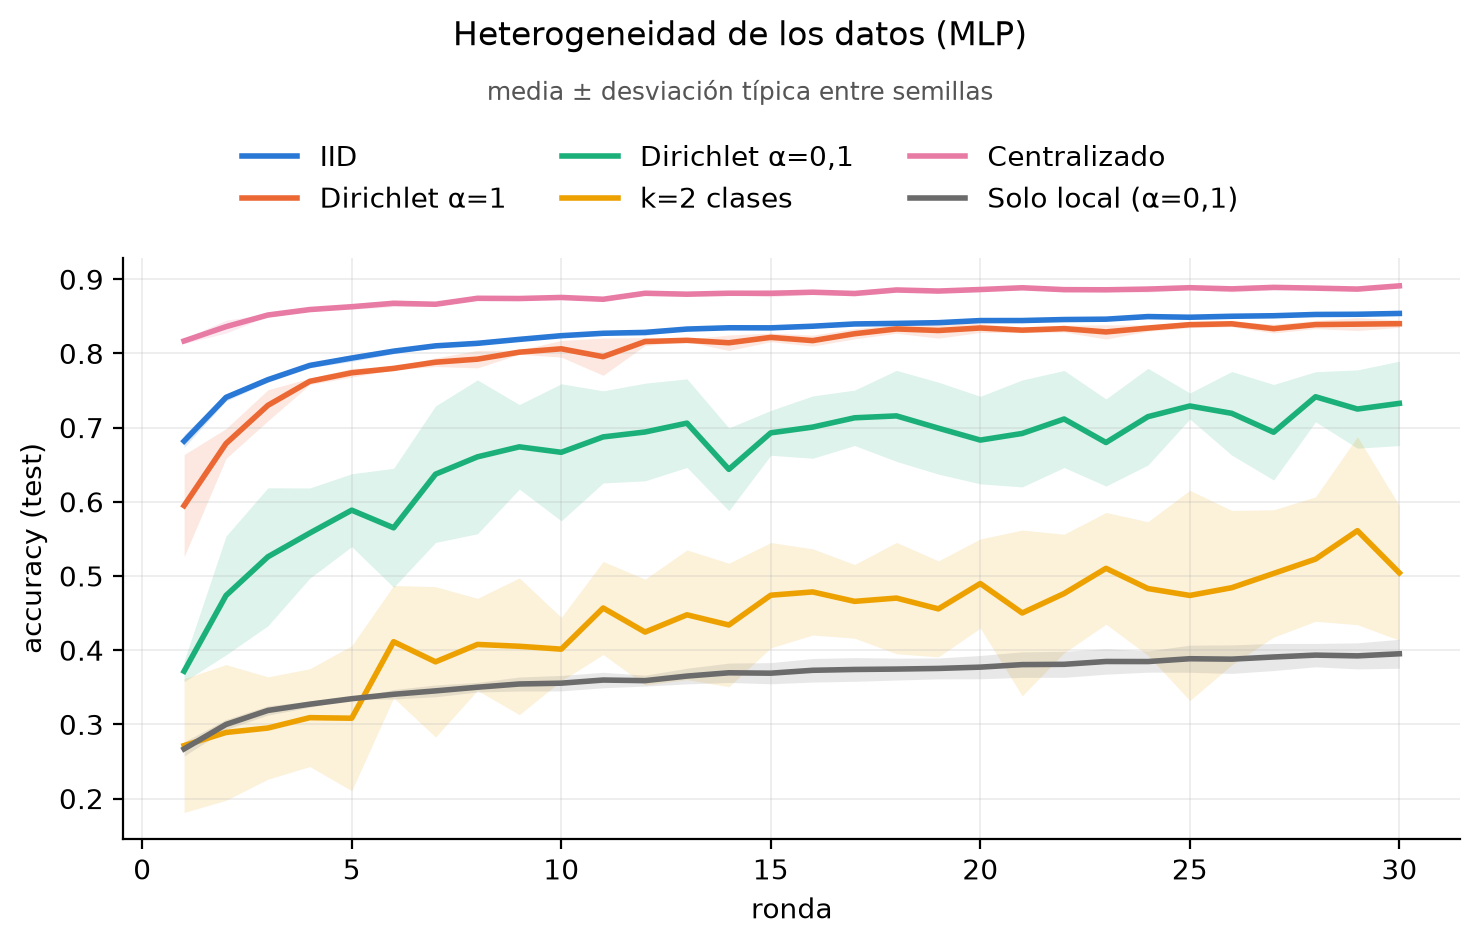
\includegraphics[width=\textwidth]{q1_accuracy.png}
    \caption{\textit{Accuracy} de test por ronda para cada reparto y las dos referencias. La línea es la media
    entre semillas y la banda, $\pm$ una desviación típica.}
    \label{fig:q1_curvas}
\end{figure}

\begin{table}[H]
    \centering
    \caption{Resultados del experimento de heterogeneidad (media $\pm$ desviación típica entre semillas)}
    \label{tab:q1}
    \setlength{\tabcolsep}{5pt}
    \begin{tabular}{lcccc}
        \hline
        Configuración & Semillas & Accuracy final & Oscilación & Salto medio \\
        \hline
        Centralizado & 3 & $0.888 \pm 0.001$ & $0.003 \pm 0.000$ & $0.003 \pm 0.000$ \\
        IID & 5 & $0.852 \pm 0.001$ & $0.003 \pm 0.001$ & $0.002 \pm 0.001$ \\
        Dirichlet $\alpha=1$ & 3 & $0.838 \pm 0.002$ & $0.006 \pm 0.003$ & $0.006 \pm 0.003$ \\
        Dirichlet $\alpha=0.1$ & 5 & $0.722 \pm 0.043$ & $0.034 \pm 0.010$ & $0.040 \pm 0.012$ \\
        Shards $k=2$ & 5 & $0.515 \pm 0.086$ & $0.061 \pm 0.030$ & $0.058 \pm 0.027$ \\
        Solo local & 3 & $0.392 \pm 0.018$ & $0.005 \pm 0.001$ & $0.003 \pm 0.001$ \\
        \hline
    \end{tabular}
\end{table}

\subsubsection{¿Cómo cambia la accuracy final y por qué?}
La \textit{accuracy} final disminuye a medida que aumenta la heterogeneidad de los datos. Básicamente 
porque a medida que la distribución de cada cliente se aleja más de la global, esta métrica empeora.
\\

Con un reparto IID, el valor esperado de la pérdida de cada cliente coincide con la pérdida global,
$\mathbb{E}[F_k(w)] = f(w)$, por lo que todas las actualizaciones locales apuntan aproximadamente hacia el mismo
óptimo y promediarlas se comporta de forma parecida a un SGD centralizado. Con $\alpha=1$ todos los clientes tienen
ejemplos de las 10 clases, aunque en proporciones desiguales, y la pérdida respecto a IID es de solo 1.4 puntos.
\\

Con $\alpha=0.1$ y $k=2$ la caída es mucho mayor (13 y 34 puntos respecto a IID). Cada cliente solo conoce una o
dos clases dominantes, de modo que el óptimo de su función local $F_k$ está lejos del óptimo global. Durante el
entrenamiento local cada modelo se desplaza hacia su propio óptimo (\textit{client drift}) y la media de estos
modelos no coincide con el óptimo de la función global. A esto se suma una convergencia más lenta: entre las
rondas 20 y 30, la curva de $\alpha=0.1$ todavía mejora 4.9 puntos frente a 1 punto en IID. Aun así, según la
teoría, aunque se aumente el número de rondas el resultado se estabiliza por debajo del de IID.
\\

El caso de $k=2$ es el más extremo, ya que la proporción Dirichlet con $\alpha=0.1$ entre las dos clases de cada
cliente hace que, en la práctica, la mayoría tenga una sola clase dominante (Figura~\ref{fig:q1_shards}). 
Además, es la configuración con mayor desviación entre semillas ($\pm 0.086$), porque el reparto depende
de la semilla.
\\

Por último, el solo local obtiene el peor resultado porque cada modelo se evalúa sobre el test global, con las 10
clases equilibradas, pero solo ha visto las pocas clases de su cliente y únicamente es capaz de predecir esas.

\begin{figure}[H]
    \centering
    \begin{minipage}{0.32\textwidth}
        \centering
        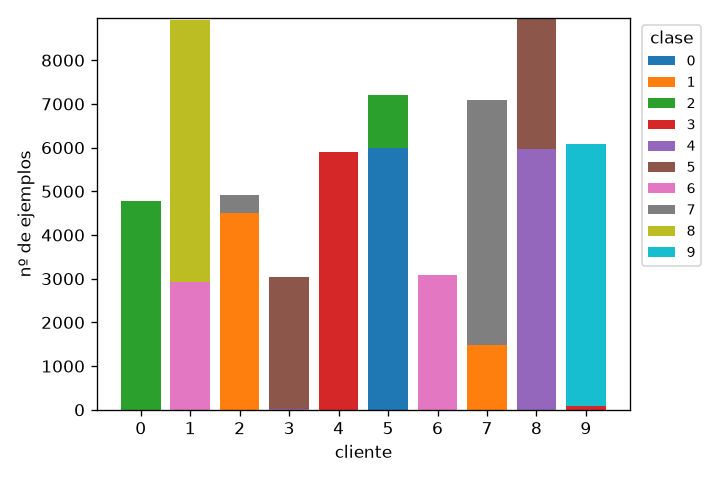
\includegraphics[width=\textwidth]{experiments/1_heterogeneidad/shards_s0.png}\\
        \small Semilla 0 (acc. $0.407$)
    \end{minipage}
    \begin{minipage}{0.32\textwidth}
        \centering
        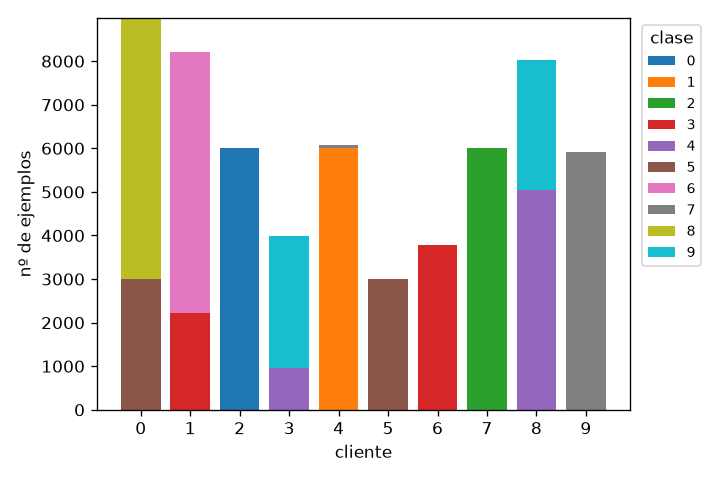
\includegraphics[width=\textwidth]{experiments/1_heterogeneidad/shards_s1.png}\\
        \small Semilla 1 (acc. $0.479$)
    \end{minipage}
    \begin{minipage}{0.32\textwidth}
        \centering
        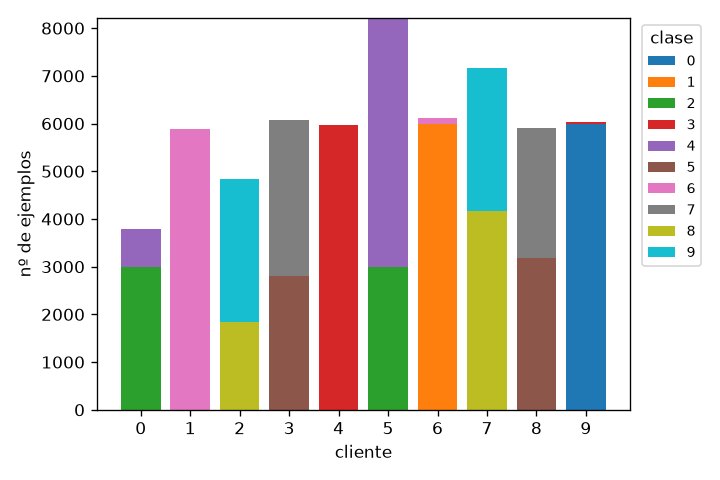
\includegraphics[width=\textwidth]{experiments/1_heterogeneidad/shards_s2.png}\\
        \small Semilla 2 (acc. $0.626$)
    \end{minipage}
    \\[0.3cm]
    \begin{minipage}{0.32\textwidth}
        \centering
        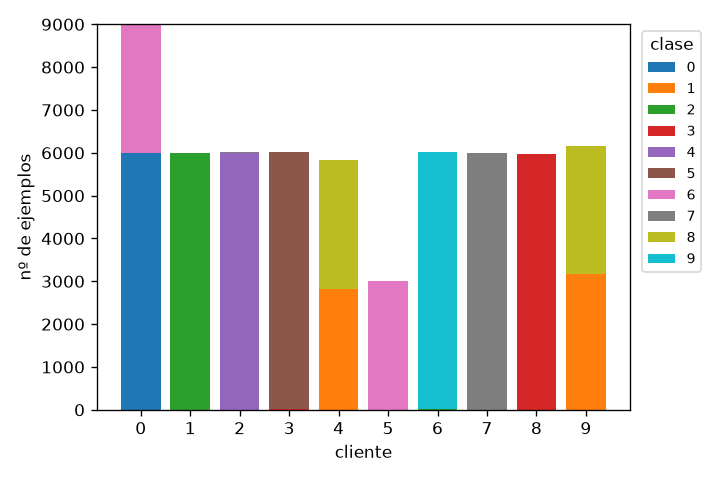
\includegraphics[width=\textwidth]{experiments/1_heterogeneidad/shards_s3.png}\\
        \small Semilla 3 (acc. $0.490$)
    \end{minipage}
    \begin{minipage}{0.32\textwidth}
        \centering
        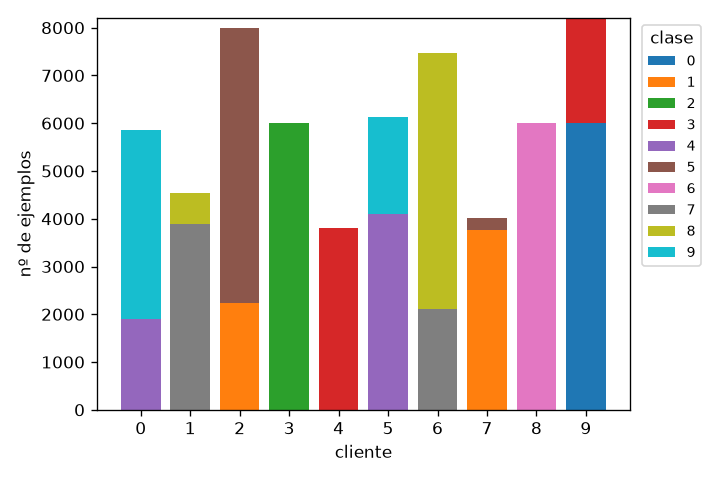
\includegraphics[width=\textwidth]{experiments/1_heterogeneidad/shards_s4.png}\\
        \small Semilla 4 (acc. $0.573$)
    \end{minipage}
    \caption{Reparto Dirichlet Shards ($k=2$, $\alpha=0.1$) con cada semilla y su \textit{accuracy} final.}
    \label{fig:q1_shards}
\end{figure}

\subsubsection{¿Cómo cambia la estabilidad de las curvas y por qué?}
El centralizado, IID y $\alpha=1$ tienen curvas suaves, con una oscilación inferior a $0.006$. Con datos IID
cualquier subconjunto de 5 clientes es representativo de la distribución global, de modo que la actualización
agregada apenas depende de qué clientes se hayan seleccionado en la ronda.
\\

En cambio, la oscilación de $\alpha=0.1$ y $k=2$ es unas 10 y 20 veces mayor que la de IID. Con $C=0.5$ los
clientes seleccionados cambian en cada ronda, y con ellos la mezcla de clases que se entrena: el modelo global se
inclina hacia las clases de los clientes elegidos y empeora en las demás, lo que produce curvas en diente de
sierra.
\\

Por último, el solo local es estable (oscilación de $0.005$) porque no hay muestreo de clientes ni agregación,
pero su curva es prácticamente plana: cada modelo solo sigue ajustando las mismas clases, por lo que en este caso
la estabilidad no indica un buen aprendizaje.

\subsection{Épocas locales}

Experimentos:
\begin{itemize}
    \item $E \in \{1, 5\}$
    \item Particionado: IID y no-IID
\end{itemize}

\subsection{Participación}

\subsection{FedAvg frente FedProx}

\subsection{Comunicación}

\subsection{CNN}